\question{10.12}{
    Soms wil men voor een getrokken steekproef beoordelen of die als representatief mag worden beschouwd met betrekking tot een bepaald kenmerk of een bepaalde variabele.
    Met de chikwadraattoets voor aanpassing kan worden getoetst of de waargenomen verdeling in dit opzicht voldoende gelijkenis vertoont met de populatieopbouw.
    Bij een opinieonderzoek over de toekomst van Europa worden $480$ kiesgerechtigde Nederlanders ondervraagd.
    Van alle ondervraagden is het opleidingsniveau genoteerd.
    In de volgende tabel wordt dit opleidingsniveau vergeleken met de totale Nederlandse bevolking:
    \begin{center}
        \renewcommand{\arraystretch}{1.25}
        \begin{tabular}{cccccc}
            \toprule
                & {\bfseries Laag} & {\bfseries Matig} & {\bfseries Redelijk} & {\bfseries Hoog} & {\bfseries Totaal} \\
            \cmidrule{1-1} \cmidrule{2-2} \cmidrule{3-3} \cmidrule{4-4} \cmidrule{5-5} \cmidrule{6-6}
                Steekproef & $134$ & $144$ & $129$ & $73$ & $480$ \\
                Populatie & $28\%$ & $36\%$ & $24\%$ & $12\%$ & $100\%$ \\
            \bottomrule
        \end{tabular}
    \end{center}
}
Toets met $\alpha=0,05$ of de steekproef als representatief mag worden beschouwd.
\answer{
    In deze opgave willen we kijken of de steekproef representatief is of niet.
    Hierbij horen de volgende nulhypothese $H_0$ en de alternatieve hypothese $H_1$:
    \begin{align*}
        H_0: &\qquad \text{de gekozen steekproef is representatief voor de populatie} \\
        H_1: &\qquad \text{de gekozen steekproef is NIET representatief voor de populatie}
    \end{align*}
    
    Verder is het significantieniveau $\alpha = 0,05$ en de steekproefdata (zie tabel) gegeven.
    Om te toetsen of de gegeven steekproefdata (observed) overeenkomen representatief zijn, moeten we allereerst de verwachte frequenties berekenen gebaseerd op de populatiepercentages.
    Dit kunnen we doen door de populatiepercentages om te rekenen naar verwachte frequenties op basis van het kiezen van $480$ kiesgerechtigde Nederlanders:

    \begin{center}
        \renewcommand{\arraystretch}{1.25}
        \begin{tabular}{ccc}
            \toprule
                {\bfseries Opleidingsniveau} & {\bfseries Steekproeffrequenties} & {\bfseries Verwachte frequenties} \\                            
                & {\bfseries (observed)} & {\bfseries (expected)} \\
            \cmidrule{1-1} \cmidrule{2-2} \cmidrule{3-3}
                Laag & $134$ & $28\% \cdot 480 = 134,4$ \\
                Matig & $144$ & $36\% \cdot 480 = 172,8$ \\
                Redelijk & $129$ & $24\% \cdot 480 = 115,2$ \\
                Hoog & $73$ & $12\% \cdot 480 = 57,6$ \\
            \cmidrule{1-1} \cmidrule{2-2} \cmidrule{3-3}
                Totaal & $480$ & $480$ \\
            \bottomrule
        \end{tabular}
    \end{center}

    Omdat we willen kijken of de geobserveerde data overeenkomen met de verwachte frequenties (van een nominale variabele), gaan we een chikwadraattoets voor aanpassing (goodness-of-fit test) uitvoeren.
    Laat $X$ een kansvariabele zijn die het aantal verwijzingen naar de afdeling intensive care telt op een willekeurige dag.
    Verder is gegeven dat er per dag $5$ orthopedische operaties zijn, die in $20\%$ van de gevallen leidt tot complicaties.
    Bij een chikwadraattoets voor aanpassing beginnen we met het defini\"eren van de nulhypothese $H_0$ en de alternatieve hypothese $H_1$.
    De verwachte frequenties zijn allemaal groter dan of gelijk aan $5$, dus kunnen we de toetsingsgrootheid direct berekenen.
    Merk op dat we de chikwadraatverdeling enkel konden gebruiken zodra de verwachte frequenties allemaal minstens $5$ zijn.
    
    De toetsingsgrootheid $X^2$ bepalen we aan de hand van de volgende formule:

    \begin{align*}
        X^2  &= \sum_{i} \frac{(O_{i} - E_{i})^2}{E_{i}},
    \end{align*}

    waarbij $i = 1,2,3,4$ de index van de kolom is.
    Dit geeft in dit specifieke geval een geobserveerde toetsingsgrootheid 
    
    \begin{align*}
        \chi^2  &= \sum_{i} \frac{(O_{i} - E_{i})^2}{E_{i}} \\
                &=\frac{(O_{1} - E_{1})^2}{E_{1}} + \frac{(O_{2} - E_{2})^2}{E_{2}} + \frac{(O_{3} - E_{3})^2}{E_{3}} + \frac{(O_{4} - E_{4})^2}{E_{4}} \\
                &= \frac{(134 - 134,4)^2}{134,4} + \frac{(144-172,8)^2}{172,8} + \frac{(129-115,2)^2}{115,2} + \frac{(73-57,6)^2}{57,6} \\
                &\approx 10,5717
    \end{align*}

    Onder de nulhypothese volgt de toetsingsgrootheid $X^2$ een chikwadraatverdeling met
    \[
        \text{df} = (\#\text{categorie\"en}-1) = 4 - 1 = 3
    \]
    vrijheidsgraden.
    Extreem grote waarde van de toetsingsgrootheid duiden op grote verschillen tussen observed en expected frequenties, dus het kritieke gebied is van de vorm $[g, \infty)$.
    Deze grenswaarde $g$ is de oplossing van de vergelijking
    \begin{align*}
        \chi^2\text{cdf}(\text{lower}=g; \text{upper}=10^{10}; \text{df}=3) = \alpha = 0,05
    \end{align*}
    De solver optie geeft $g \approx 7,8147$.
    Aangezien de toetsingsgrootheid $\chi^2$ groter dan deze grenswaarde is ($10,5717 > 7,8147$), geldt dat de toetsingsgrootheid in het kritieke gebied ligt en dus $H_0$ wordt verworpen.
    Er is voldoende bewijs om aan te nemen dat de steekproef niet representatief is voor de populatie kiesgerechtigde Nederlanders.
    
    \begin{center}
        \resizebox{0.9\textwidth}{!}{
            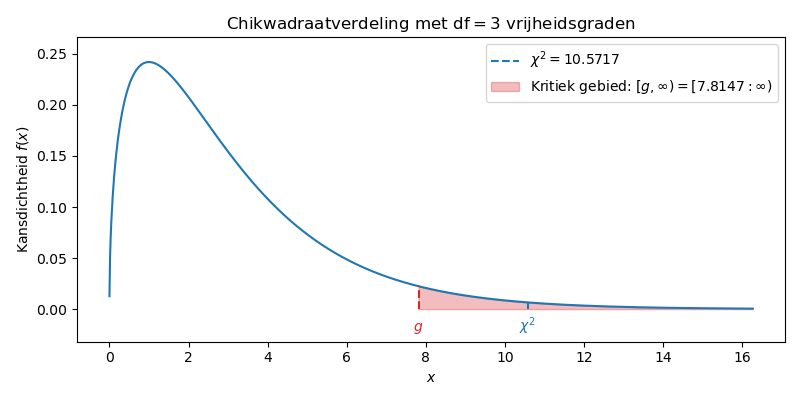
\includegraphics{opg_10.12_kritiek.png}
        }
    \end{center}

    {\bfseries Alternatief}: de $p$-waarde (rechteroverschrijdingskans) die hoort bij deze geobserveerde toetsingsgrootheid $\chi^2$ is gelijk aan
    \begin{align*}
        p   &= P(X^2 \ge \chi^2) \\
            &= \chi^2\text{cdf}(\text{lower}=\chi^2\approx 10,5717; \text{upper}=10^{10}; \text{df}=3) \\
            &\approx 0,0143
    \end{align*}

    Aangezien de $p$-waarde kleiner is dan het significantieniveau $\alpha$, betekent dit dat de geobserveerde toetsingsgrootheid $\chi^2$ een extreem hoge waarde heeft onder de aanname dat de steekproef representatief zou zijn voor de populatie.
    Dit betekent dat de nulhypothese $H_0$ wordt verworpen.
    Er is voldoende bewijs om aan te nemen dat de steekproef niet representatief is voor de populatie kiesgerechtigde Nederlanders.
    
    \begin{center}
        \resizebox{0.9\textwidth}{!}{
            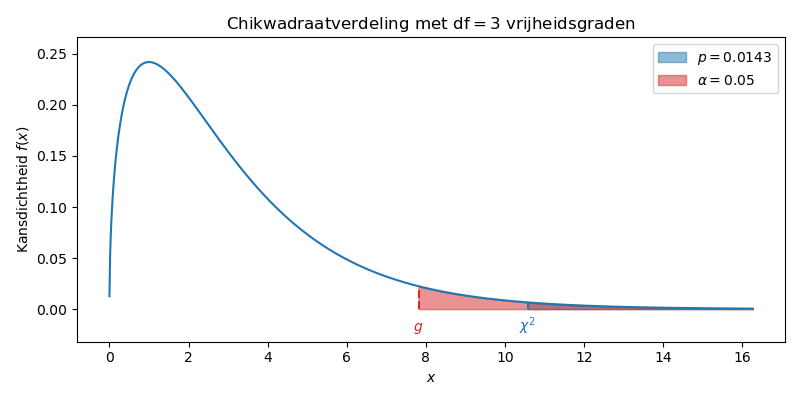
\includegraphics{opg_10.12_p_waarde.png}
        }
    \end{center}

    \vspace{1em}

    {
        \itshape \textbf{Side note:} 
        eigenlijk moet je nog doordenken over wat de toetsuitslag betekent.
        Merk op dat volgens de metingen het aantal respondenten met redelijk en hoog opleidingsniveau (veel) groter is dan verwacht, terwijl dit voor mensen met een matig opleidingsniveau een stuk lager dan verwacht is.
    }
}
